\documentclass{article}
\usepackage{graphicx}
\usepackage{placeins}
\usepackage{float}
\usepackage[acronym,nomain]{glossaries}

\makeglossaries

\begin{document}

\tableofcontents
\newpage
\printglossaries
\newpage

%%%%%%%%%%%%%%%%%%%%%%%%%%%%%%%%%%%%%%%%%%%%%%%%%%%%%%%%%%%%%%%%%%%%%%%%%%%%%%%%%%%%%%%%%
% Acronym definitions
\newacronym{sdn}{SDN}{Software Defined Network}
\newacronym{mno}{MNO}{Mobile Network Operators}
\newacronym{ngmn}{NGMN}{Next Generation Mobile Networks}
\newacronym{sil}{SIL}{Service Instance Layer}
\newacronym{nsil}{NSIL}{Network Service Instance Layer}
\newacronym{e2e}{E2E}{End to End}
\newacronym{e2e}{E2E}{End to End}
\newacronym{fh}{FH}{Fronthaul}
\newacronym{bh}{BH}{Backthaul}
\newacronym{cn}{CN}{Core Network}
\newacronym{vi}{VI}{Virtual Infrastructures}
\newacronym{IaaS}{IaaS}{Infrastructure-as-a-Service}
\newacronym{NS}{NS}{Network Services}
\newacronym{VNF}{VNF}{Virtual Network Functions}
\newacronym{MANO}{MANO}{Management and Orchestration}
\newacronym{NBI}{NBI}{Northbound Interface}
\newacronym{SBI}{SBI}{Southbound Interface}
\newacronym{MTA}{MTA}{Multi-Tenancy Application}



\section{Introduction}
Mobile networks are a key element of today's society, enabling communication, access
and information sharing. Moreover, traffic forecasts predict that the
demand for capacity will grow exponentially over the next years, mainly due to
video services. However, as cellular networks move from being voice-centric to
data-centric, operators' revenues are not able to keep pace with the predicted
increase in traffic volume. Such pressure on operators' return on investment has
pushed research efforts toward designing for 5G novel mobile network solutions
able to open the door for new revenue sources. In this context, the network
slicing paradigm has emerged as a key 5G disruptive technology addressing this
challenge.
Network slicing for 5G allows \gls{mno} to open
their physical network infrastructure platform to the concurrent deployment
of multiple logical self-contained networks, orchestrated in different ways according
to their specific service requirements; such network slices are then
(temporarily) owned by tenants. The availability of this vertical market multiplies
the monetization opportunities of the network infrastructure as new
players may come into play (e.g., automotive industry, e-health) and an higher
infrastructure capacity utilization can be achieved by admitting network slice
requests and exploiting multiplexing gains.
With network slicing for 5G networks, different services (e.g., automotive,
mobile broadband, or haptic Internet) can be provided by different network slice
instances. Each of these instances consists of a set of virtual network functions
that run on the same infrastructure with a tailored orchestration. In this way,
very heterogeneous requirements can be provided on the same infrastructure, as
different network slice instances can be orchestrated and configured separately
according to their specific requirements. Additionally, this is performed in a
cost-efficient manner as the different network slice tenants share the same
physical infrastructure.
A network slice is defined by \gls{ngmn} as “a set of network functions, and
resources to run these network functions, forming a complete instantiated
logical network to meet certain network characteristics required by the Service
Instance(s).”
According to NGMN, the concept of network slicing involves three layers,
namely, (i) service instance layer, (ii) network slice instance layer, and (iii)
resource layer. The \gls{sil} represents the end user and/or
business services provided by the operator or the third-party service providers,
which are supported by the \gls{nsil}. The NISL
is in turn supported by the resource layer, which may consist of the organic
resources such as compute, network, memory, storage, etc., or it may be more
comprehensive as being a network infrastructure, or it may be more complex
as network functions. Figure 9.1 depicts this concept where the resources at
the resource layer are dimensioned to create several sub network instances,
and network slice instances are formed that may use none, one, or multiple sub
network instances. Figure \ref{layers} depicts this concept where the resources at
the resource layer are dimensioned to create several sub network instances,
and network slice instances are formed that may use none, one, or multiple sub
network instances. 
\begin{figure}
\centering
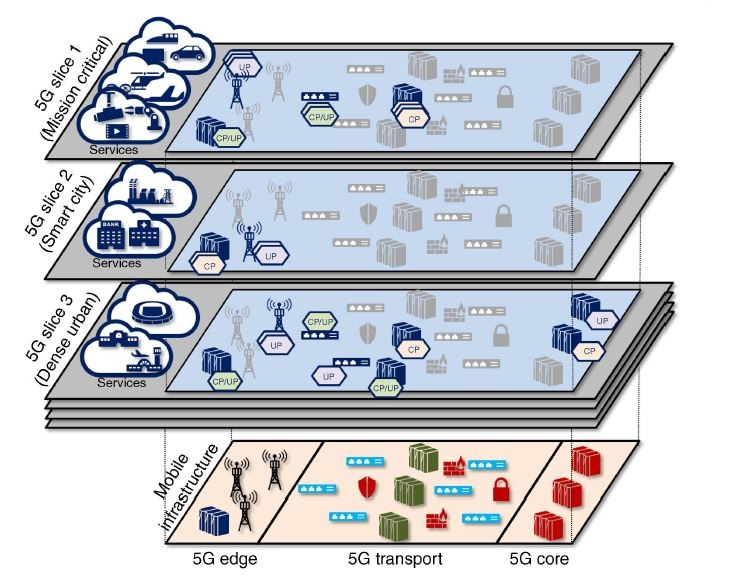
\includegraphics[scale=0.5]{pics/1.JPG}
\label{layers}
\caption{Example of network slicing in 5G.} 
\end{figure}
The end goal of network slicing in 5G mobile networks is to be able to realize
\gls{e2e} network slices starting from the mobile edge, continuing
through the mobile transport (\gls{fh} /\gls{bh}), and up until
the core network (CN). The allocation of a slice involves the selection of the
required functions, their constrained placement, the composition of the underlying infrastructure, and the allocation of the resources to fulfill the services' requirements, for example, bandwidth, latency, processing, resiliency.
We consider two main network slicing services that enable different degrees
of explicit control and are characterized by different levels of automation of the
mobile network slices management:
1) The provision of \gls{vi} under the control and operation
of different tenants-in line with an \gls{IaaS} model\footnote{form of cloud computing that provides virtualized computing resources over the internet},
that is, creation of a network slice instance.
2) The provision of tenant's owned \gls{NS}, that is, creation of a service instance.
In the former service, the deployment of a mobile network deals with the
allocation and deallocation of VIs.The logical entities within a VI encompassing
a set of compute and storage resources are interconnected by a virtual, logical
network (i.e., virtual nodes are interconnected by virtual links over the substrate
network). The Vis can be operated by the tenant via different \gls{sdn} control
models. In the latter, NS are instantiated directly over a shared infrastructure,
and as a set of interrelated \gls{VNF} connected through
one or more VNF forwarding graphs.
Multi-tenancy is an characteristic that can be applied to both
kinds of services, guaranteeing separation, isolation, and independence between
different slices coupled with the efficient sharing of the underlying resources
for both VI and NS concepts. In this context, a tenant is a logical entity owning and operating either one or more VIs or one or more network services. A tenant can be associated with an administrative entity (e.g., mobile virtual network operators) or
user of a given service (e.g., over-the-top service providers).


\newpage
\section{Architecture for Network Slicing}
The necessary architecture involves the aspects of resource virtualization, virtual infrastructure, and network service management.
\begin{figure}[h]
\centering
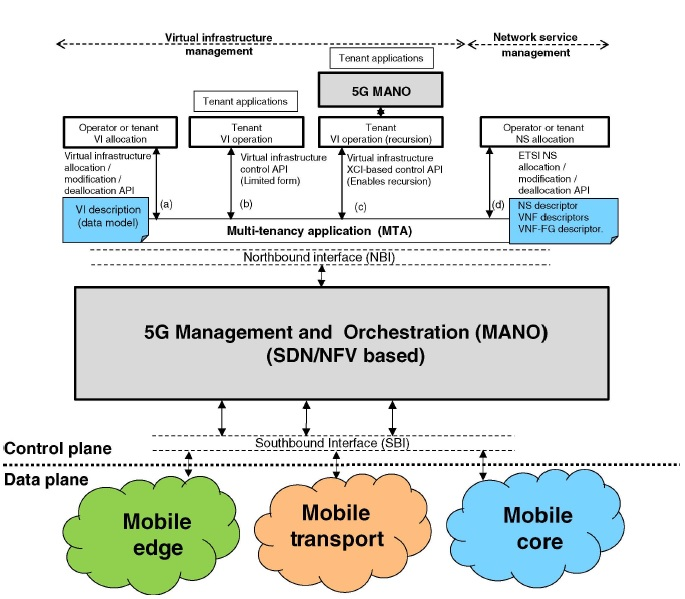
\includegraphics[scale=0.67]{pics/2.JPG}
\label{Arch}
\caption{Architecture for network slicing.} 
\end{figure}
The design proposed in Fig. \ref{Arch} follows the SDN principles of
(i) data and control plane fully decoupled, (ii) control logically centralized, and (iii) applications having an abstracted view of resources and states.
The data plane is the resource layer which includes mobile edge, mobile transport, and core. The infrastructure is composed of links, forwarding nodes (e.g., switches and routers), cloud nodes (e.g., data centers), and so on, comprising a set of network, computing, and storage resources.
The control plane is divided into two layers: an application layer at the top and the 5G \gls{MANO} platform below. The design
of the MANO is based on the ETSI management and network orchestration framework with integrated SDN-based control. The MANO
provides an abstracted view of available resources and states and control, and
management functions to an ecosystem of applications, via a \gls{NBI}. On the other hand, the MANO is connected to the data plane
elements via a \gls{SBI} to execute control and management
functions (e.g., OpenFlow, SNMP, OVSDB) on the actual hardware components.
With respect to the \gls{MTA}, it implements the
multi-tenancy support by coordinating and managing tenants access to a shared
infrastructure, performing resource isolation between instances assigned to
different tenants, and delivering multi-tenancy-related services, such as the
allocation and operation of Vis, by means of dedicated APIs in cooperation
with the data plane, enforcing this logical separation. As shown in Fig. \ref{Arch}
such APIs depend on the actual service: for the control of a VI or NS lifetime,
instantiation, modification, and deletion.

\subsection{Enablers and Design Principles}
Future 5G networks will be built on the previous novel concepts that were not envisioned by the previous generation
network architectures. The revolution provided by the introduction of software-defined networking
and network function virtualization (NFV)\footnote{NFV and VNF are often used interchangeably} opens the door to a
large list of possible applications recalling that the latter focuses primarily on optimization of the network services, instead the former to separate the control and forwarding plane for a centralized view of the network. These fundamental parts for the network slicing realization in the future 5G networks are now discussed.

\subsubsection{Modularization}
test git on linuzzz
\subsubsection{SDN-VNF}
\subsubsection{Orchestration}

\newpage

\section{Network slicing}
\subsection{Services}
\subsection{Example}
\subsection{Actual realizations}
bbbbb


\newpage
\nocite*
\bibliographystyle{plain}
\bibliography{biblist}

\end{document}